\section{Slagterieksempel}
Til at illustrere brugen af RTP, vil vi tage udgangspunkt i et aktuelt problem fra Danish Crown slagteriet. Slagteriet skal udvikle en beslutningsmodel for, hvordan en robot, skal udskære hver gris, men denne beslutning skal foretages inden grisen når robotten, hvorfor vi har et helt klassisk RTP problem. På Danish Crown slagteriet i Horsens foretages udskæringen af grise, som beskrevet på deres hjemmeside:

\begin{quote}\textit{``Grisen [\ldots] skal nu skæres i mindre, håndterbare stykker. Det sker i en meget avanceret maskine -- en såkaldt tredeler -- hvor hver halvdel af grisen deles i tre stykker: bov, mellemstykke og skinke. \\ 
\\
Robotten starter med at fotografere hver halvdel. Dataene fra billedet kombineres med ordren og kundens ønsker, hvorefter stykket deles i tre - nøjagtigt afpasset kundens ønsker.''}{ Danish Crowns hjemmeside\footnote{\url{http://www.danishcrown.dk/custom/horsens/3772.asp}}}\end{quote}

Et billede af den automatiske tredeler er vist  på \cref{fig:pig}. Problemet med den nuværende maskine er, at den ikke kan tage højde for den enkelte gris' anatomi. Omtrent 10\% af grisene har et ekstra sæt ribben, og slagteriet vil derfor gerne ændre deres udskæring til at tage højde for om dette ribben er til stede. 

\begin{figure}
 \begin{center}
  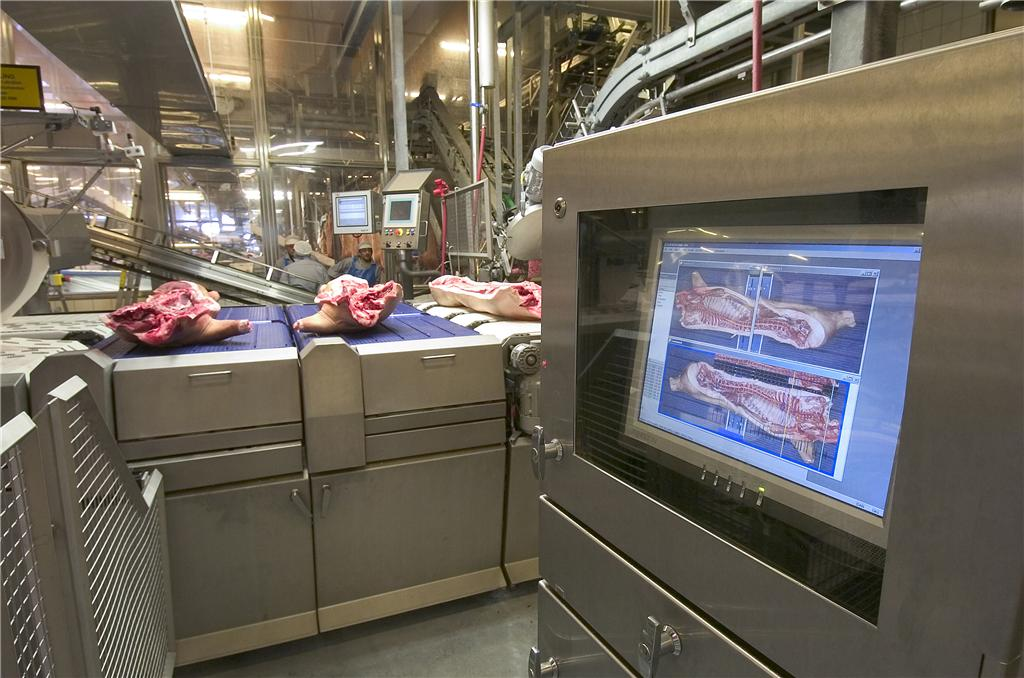
\includegraphics[scale=0.5]{images/209690-1}
	\caption{Billedet viser i forgrunden  et foto taget af tredeleren til brug for analyse. I baggrunden ses transportbåndet, hvor de halve  grise venter på på at blive udskåret af den automatisk tredeler.}
	\label{fig:pig}
\end{center}
\end{figure}


Slagteriet har placeret kameraet i starten af et transportbåndet mens udskæringsrobotten findes i den anden ende. Der kan være flere grise på transportbåndet på samme tid, og det fremfører grisene i et fast tempo. Dette giver et fast tidsrum fra grisen passerer kameraet til det passerer robotten. Vi har hermed et klassisk RTP system, hvor robotten skal foretage et valg under en hard deadline, da der skal foretages en udskæring. Før vi begynde implementeringen skal vi opdele den samlede proces i logisk afgrændsede skridt.

Vi har opdelt Arbejdsgangen i følgende skridt: 
\begin{enumerate}
\tightlist
	\item Et billede bliver taget af grisen mens den passerer kameraet.
	\item Billedet konverteres til en 3D-model af grisen.
	\item 3D-modellen analyseres.
	\item Robotten udvælger hvor udskæringerne skal være på baggrund af analysen, ordren og kundens ønske.
	\item Robotten udskærer grisen.
\end{enumerate}

Man kan se at arbejdsgangen indeholder en  række klart afgrænsede arbejdsområder, som med fordel kan modelleres som selvstændige processer i \pycsp.  Vi har derfor valgt implementere følgende processer: Kamera, Billedekonvertering, 3D-analyse og en Udskæringsproces, hvilket leder til et procesnetværk som vist i \cref{fig:pig-network}.

\begin{figure}
 \begin{center}
  
\includegraphics[scale=1]{images/pig-network}
	\caption{Procesnetværk til udskæring af grise på et slagteri.}
	\label{fig:pig-network}
\end{center}
\end{figure}

\subsubsection*{Implementering}\label{sec:deadline-exampel-implementation}
Til at implementere eksemplet i \pycsp, kan vi oprette hver gris som et objekt og tilknytte et tidspunkt som vi kan bruge som en deadline. Med denne kan hver proces evaluere om grisen har overskredet sin deadline, og i det tilfælde fjerne griseobjektet, og stoppe den videre behandling af det. Da det er ikke angivet hvordan hele processen startes,  antager vi der findes en form for detektor foran kameraet, der opfanger når en gris passerer og som dermed starter processen. 

Når detektoren starter hele processen, opretter den griseobjektet, som den sender til kameraprocessen samt sender en kopi direkte til udskæringsprocessen. Dermed ved processen, at der ankommer en gris, som den skal udskære, og hvis den inden deadline, får en analyse af grisen, kan den træffe et begrundet valg om hvordan udskæringen skal foretages. Hvis ikke denne analyse når at blive klar, bruges blot standardmodellen til at udskære grisen. \CRef{fig:pig-network2} viser et  netværk, hvor detektoren er introduceret, og som sender data til hhv. kameraprocessen og til udskæringsprocessen. 

\begin{figure}
 \begin{center}
  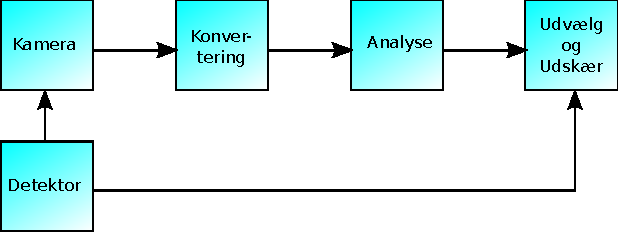
\includegraphics[scale=1]{images/pig-network2}
	\caption{Procesnetværk med detektor til initiering af hver gris.}
	\label{fig:pig-network2}
\end{center}
\end{figure}

Vi har holdt os tæt op af den virkelige verden, i designet af implementeringen men da dette er et delvist tænkt eksempel, har vi i  sagens natur ikke  adgang til slagteriet og deres maskiner, eller præcis data om grisene. Derfor må vi nødvendigvis simulere store dele af eksemplet. 

De enkelte processer foretager derfor ikke et konkret stykke arbejde, men har  tilknyttet et tal der repræsenterer det tidsrum, som vi forventer arbejdet i processen vil tage. Hver proces simulerer i stedet arbejdet, i et normalfordelt tidsrum omkring det tilknyttede tidsrum.

Detektoren starter processeringen af hver gris. Derfor står detektoren for oprettelsen af griseobjektet, hvori vi også  definerer om den har et ekstra sæt ribben. 

Det er i eksemplet  krævet, at grisen bliver udskåret mens den er indenfor robottens rækkevidde, hvorfor det er uacceptabelt hvis ikke udskæringsprocessen er aktiv i tidsrummet hvor grisen er inden for rækkevidde af robotten. 

Hvis eksemplet implementeres i \code{greenlets}-versionen, kan kun  en proces være aktiv ad gangen, og processer kan være aktive, så længe de ønsker. Dermed skal kamera-, konverterings- og analyseprocesserne frivilligt stoppe deres arbejde mens  udskæringsprocessen arbejder.  Vi har dog ikke kendskab til hvordan de processer kommer til at arbejde, og kan dermed heller ikke sige om det vil være muligt at afgive kontrollen med regelmæssige mellemrum. Selv hvis dette er muligt, findes der ikke i \pycsp mulighed for at processen stopper sit arbejde for at andre  processer kan komme til. Det bedste man vil kunne gøre, er at benytte en  \code{alternation} sammen med en \code{timeout}, for at tvinge processen til at vente et tidsrum, hvor andre processer så vil kunne komme til. Dette vil dog samtidigt sænke ydelsen af programmet da processen dermed er tvunget til at vente i tidsrummet angivet i denne \code{timeout}, selvom der ikke er andre processer klar. Hvis man vil undgå brugen af \code{timeout}, kan processerne deles op i to separate applikationer. En applikation skrevet i \pycsp der skal stå for konvertering og analyse mens en anden skal styre robotten. De to applikationer skal kunne kommunikere og  udveksle data, f.eks. igennem en database, harddisk eller anden delt datastruktur. Hvis analysen bliver færdig gemmes den i den delte datastruktur og applikationen der styrer robotten kan udnytte analysen. Hvis ikke den er klar bruges i stedet standardmodellen. Som beskrevet i \autoref{chap:csp} og som vi også kom ind på i implementeringen i \autoref{sec:des-examples}, strider en delt datastruktur dog mod ideerne i CSP, hvorfor det ikke er optimalt, men dog bedre end at sænke ydelsen af systemet ved at indsætte tvungne \code{timeouts}.

I stedet for at vælge \code{greenlets}-versionen kunne man vælge \code{processes}-versionen. Hermed vil man kunne køre processer samtidigt, og udnytte operativsystemet til at foretage preemptiv afbrydelse af processerne, således at alle processer samtidigt får en del CPU-tid. Dermed kan alle processer kører samtidigt og robotten kan foretage udskæringen. \code{Processes}-versionen risikerer dog at operativsystemet foretager et preemptivt processkift, mens udskæringsprocessen kører, således at konvertering og  analyseprocessen også kan arbejde. Potentielt vil dette kunne resultere i at grisen ikke bliver udskåret, selvom griseobjektet ankommer rettidigt til udskæringsprocessen.

Med tanke på de ovenstående fordele og ulemper der findes ved hhv.  \code{greenlets}-versionen og \code{processes}-versionen,  har vi valgt at implementere begge versioner, for i evalueringen, at sammenligne dem med RTP-versionen. 

I \code{greenlets}-versionen er udskæringsprocessen reduceret til en IO-proces der modtager griseobjekter og gemmer dem, så en anden applikation kan tilgå dem. Til dette har vi valgt at bruge en \code{dictonary} datastruktur til at gemme  hver griseobjekt under deres unikke id. Første gang processen modtager et griseobjekt vil det være ubehandlet, men gemmes i datastrukturen for at indikere at et tilsvarende objekt er ved at blive behandlet i proces-netværket. Såfremt griseobjektet bliver færdigbehandlet indenfor sin deadline, vil det færdigbehandlede griseobjekt modtages fra analyseprocessen, og overskrive det ubehandlede griseobjekt. Hvis det ikke når at blive færdigbehandlet, vil den anden applikation stadig kunne tilgå det ubehandlede griseobjekt, og derved vide at en gris skal udskæres. 

\code{Processes}-versionen, er magen til \code{greenlets}-versionen, men den praktiske forskel at processerne kører som selvstændige python-processer og derfor har muligheden for parallel kørsel. 

%\subsection{Eksempel 2 - Sensornetværk med høj/lav -prioritet}
%eks2: skal vise alternation, kan være en sensor som modtager måledata med lav prioritet og som skal sende måledata på opdordring med høj prioritet.
